\def\languageisfrench{}

\documentclass[a4paper,10pt]{article}

\usepackage[a4paper, top=2.5cm, bottom=2.2cm, left=2.2cm, right=2.2cm]{geometry} % Marge reduction.

\ifdefined\languageisfrench
	%% Language specific package
	\usepackage[french]{babel}
	\frenchbsetup{StandardLists=true} % Necessary to use enumitem with babel/french.
\fi

%% Font and typing packages
\usepackage{fontspec}
\setmainfont[
	Ligatures=TeX,
	SmallCapsFont={PT Serif}
	]{PT Serif} % default is Latin Modern
\newfontfamily\antiquefont[Ligatures=TeX]{Caslon Antique} % fancy font
\usepackage{microtype}			% Greatly improves general appearance of the text.
\usepackage{SIunits}			% Unit appearance.
\usepackage{ulem}				% To cross words out. Use \sout{}.

%% Array utilities
\usepackage{array}				% Additionnal options for arrays.
\usepackage{colortbl}			% Additionnal options for coloring arrays.
\usepackage[table]{xcolor}		% Auto alternate grey-white rows.
\usepackage[export]{adjustbox}		% Centered pics in tables
\usepackage{slashbox}		% diagonal slash in a cell

%% List utilities
\usepackage[inline]{enumitem}   % Display inline lists.
\usepackage{etoolbox}           % General utility. Good for lists for instance.
\usepackage{xparse}             % List utilities.

%% Frames
\usepackage{framed}				% Boxes.
\usepackage[framemethod=TikZ]{mdframed}% For fancy frames.
\usepackage{tikz}				% For fancy frames.
\usepackage{wrapfig}			% Fancy insertion of pics in text.

%% Page utilities
\usepackage{parskip} 			% no paragraph indentation and spaces between paragraphs.
\usepackage{multicol}			% Allows to divide a part of the page in multiple columns.
\usepackage{titlesec} 			% titles customization
\usepackage{caption}			% captions customization
\usepackage{fancyhdr}		% For custom headers and foot texts
\pagestyle{fancy}
	
%% Others
\usepackage{xstring}            % String parsing, cutting, etc.
\usepackage{xr}					% for FAQ cross-referencing
\usepackage[hidelinks, bookmarks=false, pdfdisplaydoctitle=true, pdfstartview=FitH, pdfpagelabels=false]{hyperref} % Links in PDF.

\makeatletter

%%% Language specific stuff

\ifdefined\languageisfrench
	
\newcommand{\translationteam}{\item \og AEnoriel \fg \item \og Anglachel \fg \item \og Astadriel \fg \item \og Batcat \fg \item \og Bigfish \fg \item \og Eru \fg  \item \og Gandarin \fg \item \og Groumbahk \fg \item \og Iluvatar \fg \item \og Mammstein \fg \item \og Shlagrabak \fg \item et beaucoup d'autres...}

\hypersetup{
	pdfauthor={Équipe de traduction française de T9A},
	pdfsubject={Règles pour le jeu Batailles Fantastiques : Le 9\ieme{} Âge},
}

%%% Commands %%%

\ifdef{\isitanAB}{

\newcommand{\addtosortedlist}[1]{%
	\protected@edef\textarg{#1}%
	\protected@edef\textwithoutspaces{\expandafter\removespaces\expandafter{\textarg}}%
	\substitute\textwithoutspaces{É}{E}% Most used special characters of the language, and equivalent for alphabetical ordering
	\substitute\textwithoutspaces{È}{E}%
	\substitute\textwithoutspaces{Ê}{E}%
	\substitute\textwithoutspaces{é}{e}%
	\substitute\textwithoutspaces{è}{e}%
	\substitute\textwithoutspaces{ê}{e}%
	\substitute\textwithoutspaces{À}{A}%
	\substitute\textwithoutspaces{à}{a}%
	\substitute\textwithoutspaces{ù}{u}%
	\expandafter\sortitem\expandafter[\textwithoutspaces]{#1}%
}%

\newcommand{\pts}[1]{% First step is to remove spaces if there are some
	\def\numberwithoutspaces{\expandafter\removespaces\expandafter{#1}}%
	% Next step is getting rid of formatting if there are any (bold, color, ...)
	\pdfstringdef\cleannumber{\numberwithoutspaces}%
	% Now we can try if it is 1 or not
	\expandafter\ifstrequal\expandafter{\cleannumber}{1}{#1~\labels@point}{%
	\expandafter\ifstrequal\expandafter{\cleannumber}{0.5}{0,5~\labels@point}{%
	\expandafter\ifstrequal\expandafter{\cleannumber}{1.5}{1,5~\labels@point}{%
	#1~\labels@points}}}%
}

}{}

% Dark gods
\newcommand{\dchange}{Changement}
\newcommand{\dlust}{Luxure}
\newcommand{\pestilence}{Pestilence}
\newcommand{\wrath}{Courroux}
\newcommand{\truechaos}{Chaos Primordial}


% Nothing to edit here

\ifdef{\isitanAB}{

\newcommand{\alliancepts}[1]{
\ifsubstring{#1}{\free}{%
		\free{}%
	}{%
	\ifsubstring{#1}{\permodel}{%
		\splitatinf{#1}\myoption\myvalue%
		\pts{\myvalue}\permodel{}%
	}{%
	\pts{#1}
	}}
}

% You might wanna change the order of the gods - advanced user
\newcommand{\allianceoptions}[1]{%
	\defallianceoptions{#1}%
	\unitentryformat{\labels@allianceoptions\spacebeforecolon{}:}\newline
	\expandafter\ifblank\expandafter{\allianceoptions@introsentence}{}{\noindent\allianceoptions@introsentence{}\spacebeforecolon{}:}
	
	\expandafter\ifblank\expandafter{\allianceoptions@wrath}{
		\setlength{\columnseprule}{0.5pt}
		\renewcommand{\columnseprulecolor}{\color{black!30}}
		\vspace*{-0.2cm}\begin{multicols}{3}\raggedcolumns
		
			\begin{center}
			\noindent\dchange{}
			
			\noindent\alliancepts{\allianceoptions@change}
			\vspace*{-0.3cm}
			\end{center}
		
		\columnbreak
		
			\begin{center}
			\noindent\dlust{}
			
			\noindent\alliancepts{\allianceoptions@lust}
			\vspace*{-0.3cm}
			\end{center}
		
		\columnbreak

			\begin{center}
			\noindent\pestilence{}
			
			\noindent\alliancepts{\allianceoptions@pestilence}
			\vspace*{-0.3cm}
			\end{center}
			
		\end{multicols}
		\setlength{\columnseprule}{0pt}	
	}{
		\setlength{\columnseprule}{0.5pt}
		\renewcommand{\columnseprulecolor}{\color{black!30}}
		\vspace*{-0.2cm}\begin{multicols}{4}\raggedcolumns
		
			\begin{center}
			\noindent\dchange{}
			
			\noindent\alliancepts{\allianceoptions@change}
			\vspace*{-0.3cm}
			\end{center}
		
		\columnbreak

			\begin{center}
			\noindent\wrath{}
			
			\noindent\alliancepts{\allianceoptions@wrath}
			\vspace*{-0.3cm}
			\end{center}
		
		\columnbreak
		
			\begin{center}
			\noindent\dlust{}
			
			\noindent\alliancepts{\allianceoptions@lust}
			\vspace*{-0.3cm}
			\end{center}
		
		\columnbreak

			\begin{center}
			\noindent\pestilence{}
			
			\noindent\alliancepts{\allianceoptions@pestilence}
			\vspace*{-0.3cm}
			\end{center}
			
		\end{multicols}
		\setlength{\columnseprule}{0pt}
	}
}

}{}


%%% Labels %%%

% Profile

\newcommand{\labels@M}{M}
\newcommand{\labels@WS}{CC}
\newcommand{\labels@BS}{CT}
\newcommand{\labels@S}{F}
\newcommand{\labels@T}{E}
\newcommand{\labels@W}{PV}
\newcommand{\labels@I}{I}
\newcommand{\labels@A}{A}
\newcommand{\labels@Ld}{Cd}
\newcommand{\labels@Invocation}{Invocation} % For Vampire Covenant profiles
\newcommand{\labels@roundbase}{rond} % printed after XX mm for round bases

\newcommand{\Strength}{Force}

% Technical

\newcommand{\labels@range}{Portée}
\newcommand{\labels@point}{pt}
\newcommand{\labels@points}{pts}
\newcommand{\labels@only}{uniquement}
\newcommand{\labels@magic}{Magie}
\newcommand{\labels@pathsused}{Génère ses sorts dans la Discipline}
\newcommand{\labels@model}{figurine}
\newcommand{\labels@models}{figurines}
\newcommand{\labels@Singlemodel}{Figurine \textbf{seule}}

% Unit entry labels

\newcommand{\labels@basesize}{Socle}
\newcommand{\labels@trooptype}{Type de troupe}
\newcommand{\labels@specialrules}{Règles Spéciales}
\newcommand{\labels@alignment}{Allégeance}
\newcommand{\labels@alliance}{Allégeance}
\newcommand{\labels@allianceoptions}{Options d'Allégeance}
\newcommand{\labels@greenhiderace}{Race de Peaux Vertes}
\newcommand{\labels@equipment}{Équipement}
\newcommand{\labels@weapons}{Armes}
\newcommand{\labels@armour}{Armure}
\newcommand{\labels@options}{Options}
\newcommand{\labels@commandgroup}{État-Major}
\newcommand{\labels@charactermounts}{Montures de Personnages}
\newcommand{\labels@mounts}{Montures}
\newcommand{\labels@mount}{Monture}
\newcommand{\labels@specialequipment}{Équipement Spécial}

% Command groups

\newcommand{\labels@champion}{Champion}
\newcommand{\labels@standardbearer}{Porte-Étendard}
\newcommand{\labels@musician}{Musicien}
\newcommand{\labels@singlebannerallowance}{Une seule unité de ce type peut prendre une Bannière Magique}
\newcommand{\labels@condsinglebannerallowance}{Une seule unité de ce type peut prendre une Bannière Magique si}
\newcommand{\labels@bannerallowance}{Bannière Magique}
\newcommand{\labels@veteranstandardbearer}{Peut devenir Porte-Étendard Vétéran}
\newcommand{\labels@championallowance}{Arme Magique}

% Titles

\newcommand{\labels@armylist}{Liste des Troupes}
\newcommand{\labels@lords}{Seigneurs}
\newcommand{\labels@heroes}{Héros}
\newcommand{\labels@coreunits}{Unités de Base}
\newcommand{\labels@specialunits}{Unités Spéciales}
\newcommand{\labels@rareunits}{Unités Rares}
\newcommand{\labels@armywiderules}{Règles Communes de l'Armée}
\newcommand{\labels@armyspecialrules}{Règles Spéciales de l'Armée}
\newcommand{\labels@armoury}{Armurerie}
\newcommand{\labels@magicalitems}{Objets Magiques}
\newcommand{\labels@magicalweapons}{Armes Magiques}
\newcommand{\labels@magicalarmour}{Armures Magiques}
\newcommand{\labels@talismans}{Talismans}
\newcommand{\labels@enchanteditems}{Objets Enchantés}
\newcommand{\labels@arcaneitems}{Objets Cabalistiques}
\newcommand{\labels@magicalbanners}{Bannières Magiques}
\newcommand{\labels@quickrefsheet}{Fiche de Référence}
\newcommand{\labels@changelog}{Change Log}

\newcommand{\labels@lordsInitial}{S}
\newcommand{\labels@heroesInitial}{H}
\newcommand{\labels@coreunitsInitial}{B}
\newcommand{\labels@specialunitsInitial}{S}
\newcommand{\labels@rareunitsInitial}{R}
\newcommand{\labels@mountsInitial}{M}


% Titlepage

\newcommand{\labels@fantasybattles}{Batailles Fantastiques}
\newcommand{\labels@NinthAge}{Le 9\ieme{} Âge}
\newcommand{\labels@armyrules}{Règles de l'Armée}
\newcommand{\labels@frontpagecredits}{%
\labels@fantasybattles{} : \labels@NinthAge{} est un jeu créé et entretenu par la communauté qui met en scène des affrontements de figurines.\newline
Toutes les règles sont disponibles gratuitement sur le site suivant. Vos retours et suggestions sont les bienvenus : \url{http://www.the-ninth-age.com/}
}
\newcommand{\labels@license}{Copyright Creative Commons license : \url{the-ninth-age.com/license.html}}
\newcommand{\labels@tableofcontents}{Sommaire}
\newcommand{\labels@introduction}{%
\begin{center}\noindent{\Largerfontsize\textbf{Note des traducteurs}}\end{center}
\vspace{0.5cm}

Nous souhaitons remercier chaleureusement l'équipe à l'initiative du 9\ieme{} Âge pour leur motivation et leur travail continu pour faire vivre notre passion. Nous espérons que ce jeu saura développer les qualités pour plaire au plus grand nombre et réunir les joueurs, amateurs comme habitués des tournois, autour de règles amusantes et équilibrées, pour finalement s'imposer comme un standard du jeu de figurines. Une grande ambition qui ne pourra s'accomplir que \textbf{grâce à vous}, la communauté, via des retours constructifs, afin de modeler le jeu selon nos désirs. N'étant \textbf{en aucun cas à but lucratif}, le 9\ieme{} Âge part avec un avantage considérable. Les règles des éventuelles nouvelles sorties ne sont pas dictées par le besoin de vendre ces nouveautés. Vous pouvez choisir et acheter vos figurines où bon vous semble, il n'y a pas un unique revendeur toléré. Enfin, vous pouvez être assurés que tant que le 9\ieme{} Âge sera joué, vous disposerez d'un \textbf{support continu et régulier}, celui-ci étant offert par la communauté.

Concernant la traduction en elle-même, nous avons fait de notre mieux pour vous offrir une version de qualité, dont nous espérons qu'elle surpasse celle de la version originale ! Si vous constatez des coquilles, des erreurs, merci de nous les signaler en nous contactant sur le forum du 9\ieme{} Âge, dans le \textbf{sous-forum français} (\url{http://www.the-ninth-age.com/index.php?board/117-french/}). Vous y trouverez aussi les dernières mises à jour. \textbf{En cas de conflit d'interprétation avec la version originale, la version originale fait référence}.

\vspace{0.5cm}
Que ce jeu vous apporte d'innombrables heures de plaisir partagé !

\vspace{1cm}

\ifdef{\translationteam}{
	\begin{multicols}{3}
	\begin{itemize}
		\translationteam
	\end{itemize}
	\end{multicols}
}{}
}
\newcommand{\labels@rulechanges}{% blank ATM
}
\newcommand{\labels@latexcredit}{Document réalisé à l'aide de \LaTeX .}


%%% Technical commands

\newcommand{\only}[1]{(#1 uniquement)}
\newcommand{\free}{gratuit}
\newcommand{\upto}{jusqu'à}
\newcommand{\Upto}{Jusqu'à}
\newcommand{\unlimited}{pas de limite}
\newcommand{\permodel}{/fig.}
\newcommand{\listlastchoice}{ ou}
\newcommand{\notif}[1]{(pas #1)}
\newcommand{\wordand}{et}
\newcommand{\wordwith}{avec}
\newcommand{\ifNmodelsorless}[1]{(#1 figurines ou moins)}
\newcommand{\unitwith}{unité avec}
\newcommand{\From}{De} % From ... to ... models
\newcommand{\wordto}{à}
\newcommand{\wordAll}{Tous}
\newcommand{\spacebeforecolon}{ } % French put a space before colons
\newcommand{\minprice}{Coût min. :}
\newcommand{\mincostfor}{Coût min. pour}
\newcommand{\maxunitsize}{Taille max.}
\newcommand{\additionalfigscost}{Les figurines additionnelles coûtent}


%%% Special rules %%%

\newcommand{\ambush}{Embuscade}
\newcommand{\armourpiercing}[1]{Perforant\ifblank{#1}{}{ (#1)}}
\newcommand{\bodyguard}[1]{Garde du Corps\ifblank{#1}{}{ (#1)}}
\newcommand{\breathweapon}[1]{Attaque de Souffle\ifblank{#1}{}{ (#1)}}
\newcommand{\channel}{Canalisation}
\newcommand{\crushattack}{Attaque Écrasante}
\newcommand{\daemonicinstability}{Instabilité Démoniaque}
\newcommand{\devastatingcharge}{Charge Dévastatrice}
\newcommand{\distracting}{Distrayant}
\newcommand{\divineattacks}{Attaques Divines}
\newcommand{\engineer}{Ingénieur}
\newcommand{\ethereal}{Éthéré}
\newcommand{\fastcavalry}{Cavalerie Légère}
\newcommand{\fear}{Peur}
\newcommand{\fightinextrarank}{Combat avec un Rang Supplémentaire}
\newcommand{\fireborn}{Né du Feu}
\newcommand{\flamingattacks}{Attaques Enflammées}
\newcommand{\flammable}{Inflammable}
\newcommand{\frenzy}{Frénésie}
\newcommand{\fly}[1]{Vol\ifblank{#1}{}{ (#1)}}
\newcommand{\grindingattacks}[1]{Attaques de Broyage\ifblank{#1}{}{ (#1)}}
\newcommand{\hardtarget}{Camouflé}
\newcommand{\hatred}{Haine}
\newcommand{\hellfire}{Feu Démoniaque}
\newcommand{\hidden}{Caché}
\newcommand{\holyattacks}{Attaques Divines} % deprecated, still has to be filled. same as Divine Attacks.
\newcommand{\immunetopsychology}{Immunisé à la Psychologie}
\newcommand{\impacthits}[1]{Touches d'Impact\ifblank{#1}{}{ (#1)}}
\newcommand{\insignificant}{Insignifiant}
\newcommand{\largetarget}{Grande Cible}
\newcommand{\lethalstrike}{Coup Fatal}
\newcommand{\lightningattacks}{Attaques Foudroyantes}
\newcommand{\lightningreflexes}{Réflexes Foudroyants}
\newcommand{\lighttroops}{Troupe Légère}
\newcommand{\magicresistance}[1]{Résistance à la Magie\ifblank{#1}{}{ (#1)}}
\newcommand{\magicalattacks}{Attaques Magiques}
\newcommand{\metalshifting}{Fusion du Métal}
\newcommand{\moveorfire}{Mouvement ou Tir}
\newcommand{\multipleshots}[1]{Tirs Multiples\ifblank{#1}{}{ (#1)}}
\newcommand{\multiplewounds}[2]{Blessures Multiples\ifblank{#1}{}{ (#1\ifblank{#2}{)}{, #2)}}}
\newcommand{\notaleader}{Pas un Meneur}
\newcommand{\otherworldly}{D'Outre-Monde}
\newcommand{\pathmaster}[1]{Maître de la Voie\ifblank{#1}{}{ (#1)}}
\newcommand{\poisonedattacks}{Attaques Empoisonnées}
\newcommand{\quicktofire}{Tir Rapide}
\newcommand{\randommovement}[1]{Mouvement Aléatoire\ifblank{#1}{}{ (#1)}}
\newcommand{\randomattacks}[1]{Attaques Aléatoires\ifblank{#1}{}{ (#1)}}
\newcommand{\regeneration}[1]{Régénération\ifblank{#1}{}{ (#1+)}}
\newcommand{\reload}{Rechargez !}
\newcommand{\requirestwohands}{Arme à deux Mains}
\newcommand{\scythes}{Faux}
\newcommand{\scout}{Éclaireur}
\newcommand{\scouts}{Éclaireurs}
\newcommand{\stomp}[1]{Piétinement\ifblank{#1}{}{ (#1)}}
\newcommand{\strider}[1]{Guide\ifblank{#1}{}{ (#1)}}
\newcommand{\stubborn}{Tenace}
\newcommand{\stupidity}{Stupidité}
\newcommand{\skirmisher}{Tirailleur}
\newcommand{\skirmishers}{Tirailleurs}
\newcommand{\sweepingattack}{Attaque au Passage}
\newcommand{\swiftstride}{Course Rapide}
\newcommand{\thunderouscharge}{Charge Tonitruante}
\newcommand{\terror}{Terreur}
\newcommand{\toxicattacks}{Attaques Toxiques}
\newcommand{\unbreakable}{Indémoralisable}
\newcommand{\undead}{Mort-Vivant}
\newcommand{\unstable}{Instable}
\newcommand{\unwieldy}{Encombrant}
\newcommand{\vanguard}{Avant-Garde}
\newcommand{\volleyfire}{Tir de Volée}
\newcommand{\warplatform}{Plateforme de Guerre}
\newcommand{\wardsave}[1]{Sauvegarde Invulnérable\ifblank{#1}{}{ (#1+)}}
\newcommand{\weaponmaster}{Maître d'Ar\-mes}
\newcommand{\wizardconclave}[1]{Conclave de Sorciers\ifblank{#1}{}{ (#1)}}


%%% Magic %%%


% General

\newcommand{\Pathof}{Voie}

\newcommand{\battle}{Commune}

\newcommand{\anyofthebattlemagic}{dans n'importe laquelle des Voies Communes}
\newcommand{\ONLYanyofthebattlemagic}{Commune de votre choix}

\newcommand{\magiclevel}[1]{\ifnumcomp{#1}{<}{3}{Apprenti Magicien}{Maître Magicien} Niveau #1}
\newcommand{\Level}{Niveau}

\newcommand{\wizard}{Magicien}
\newcommand{\wizards}{Magiciens}

\newcommand{\learnedspell}{Sort Appris}
\newcommand{\learnedspells}{Sorts Appris}
\newcommand{\attributespell}{Attribut de la Voie}
\newcommand{\attributespells}{Attributs de la Voie}
\newcommand{\attributespellnumber}{A}
\newcommand{\traitspell}{Sort Caractéristique}
\newcommand{\traitspells}{Sorts Caractéristiques}
\newcommand{\traitspellnumber}{C}


\newcommand{\boundspell}[1]{Objet de Sort\ifblank{#1}{}{, Puissance #1}}
\newcommand{\boundspells}[1]{Objets de Sort\ifblank{#1}{}{, Puissance #1}}

% Casting Vocabulary

\newcommand{\lostfocus}{Perte de Concentration}
\newcommand{\miscast}{Fiasco}
\newcommand{\miscasts}{Fiascos}
\newcommand{\overwhelmingpower}{Pouvoir Irrésistible}

\newcommand{\breachintheveil}{Brèche dans le Voile}
\newcommand{\catastrophicdetonation}{Explosion Catastrophique}
\newcommand{\witchfire}{Feu de Sorcières}
\newcommand{\sorcerousbacklash}{Contrecoup Magique}
\newcommand{\amnesia}{Amnésie}

% Spell Types

\newcommand{\augment}{Amélioration}
\newcommand{\hex}{Malédiction}
\newcommand{\universal}{Universel}
\newcommand{\missile}{Projectile}
\newcommand{\damage}{Dégâts}
\newcommand{\direct}{Direct}
\newcommand{\focused}{Focalisé}
\newcommand{\vortex}{Vortex}
\newcommand{\ground}{Marqueur}
\newcommand{\linetemplate}{Gabarit de Ligne}
\newcommand{\specialTYPE}{Spécial}
\newcommand{\aura}{Aura}
\newcommand{\castersunit}{Unité du Lanceur}
\newcommand{\caster}{Lanceur}

\newcommand{\template}{Gabarit}

% Spell Durations

\newcommand{\lastsoneturn}{Dure un Tour}
\newcommand{\instant}{Immédiat}
\newcommand{\permanent}{Permanent}
\newcommand{\remainsinplay}{Reste en Jeu}


% Battle Magic

\newcommand{\alchemy}{de l'Alchimie}
\newcommand{\alchemyattribute}{Édit de Fer}
\newcommand{\alchemysignature}{Métal Fondu}
\newcommand{\alchemyspellone}{Lames Enchantées}
\newcommand{\alchemyspelltwo}{Corrosion Rampante}
\newcommand{\alchemyspellthree}{Manteau de Vif-Argent}
\newcommand{\alchemyspellfour}{Pieu d'Argent}
\newcommand{\alchemyspellfive}{Fléau de l'Acier}
\newcommand{\alchemyspellsix}{Transmutation en Or}

\newcommand{\death}{de la Mort}
\newcommand{\deathattribute}{Nuage de Désespoir}
\newcommand{\deathsignature}{Le Baiser de la Faucheuse}
\newcommand{\deathspellone}{Malédiction du Mortel}
\newcommand{\deathspelltwo}{Esprits Dévorants}
\newcommand{\deathspellthree}{Sangsue Psychique}
\newcommand{\deathspellfour}{Moisson d’Âmes}
\newcommand{\deathspellfive}{L’Abîme aussi te Regarde...}
\newcommand{\deathspellsix}{Maelström d’Âmes}

\newcommand{\fire}{du Feu}
\newcommand{\fireattribute}{Feu Déchaîné}
\newcommand{\firesignature}{Boule de Feu}
\newcommand{\firespellone}{Cascade Ardente}
\newcommand{\firespelltwo}{Épées Flamboyantes}
\newcommand{\firespellthree}{Jet de Flammes}
\newcommand{\firespellfour}{Traits Enflammés}
\newcommand{\firespellfive}{Remparts Incandescents}
\newcommand{\firespellsix}{Souffler sur les Braises}

\newcommand{\heavens}{des Cieux}
\newcommand{\heavensattribute}{Second Sceau}
\newcommand{\heavenssignature}{Aquilon}
\newcommand{\heavensspellone}{Bourrasque}
\newcommand{\heavensspelltwo}{Choc Foudroyant}
\newcommand{\heavensspellthree}{Conjonction Astrale}
\newcommand{\heavensspellfour}{Fléau du Ponant}
\newcommand{\heavensspellfive}{Déluge d'Éclairs}
\newcommand{\heavensspellsix}{Appel de la Comète}

\newcommand{\light}{de la Lumière}
\newcommand{\lightattribute}{Lumière Gardienne}
\newcommand{\lightsignature}{Éclat Brûlant}
\newcommand{\lightspellone}{Bouclier Protecteur}
\newcommand{\lightspelltwo}{Étincelle de Courage}
\newcommand{\lightspellthree}{Vitesse Fulgurante}
\newcommand{\lightspellfour}{Toile Scintillante}
\newcommand{\lightspellfive}{Distorsion Temporelle}
\newcommand{\lightspellsix}{Bannissement Divin}

\newcommand{\nature}{de la Nature}
\newcommand{\natureattribute}{Souffle de Vie}
\newcommand{\naturesignature}{Eaux Vivifiantes}
\newcommand{\naturespellone}{Maître de la Terre}
\newcommand{\naturespelltwo}{Le Trône de Chêne}
\newcommand{\naturespellthree}{Esprits des Bois}
\newcommand{\naturespellfour}{Croissance Estivale}
\newcommand{\naturespellfive}{Peau Rocailleuse}
\newcommand{\naturespellsix}{Créatures Souterraines}

\newcommand{\shadows}{des Ombres}
\newcommand{\shadowsattribute}{Course Parmi les Ombres}
\newcommand{\shadowssignature}{Miasmes Obscurs}
\newcommand{\shadowsspellone}{Orbe de Noirceur}
\newcommand{\shadowsspelltwo}{Partir en Fumée}
\newcommand{\shadowsspellthree}{Expérience de Mort Imminente}
\newcommand{\shadowsspellfour}{Char Vaporeux}
\newcommand{\shadowsspellfive}{Ombres Dévorantes}
\newcommand{\shadowsspellsix}{Scalpel Psychique}

\newcommand{\wilderness}{de la Sauvagerie}
\newcommand{\wildernessattribute}{La Chasse Sauvage}
\newcommand{\wildernesssignature}{La Bête qui Sommeille}
\newcommand{\wildernessspellone}{Essaim d’Insectes}
\newcommand{\wildernessspelltwo}{Rage Intérieure}
\newcommand{\wildernessspellthree}{Pieu de Rougebois}
\newcommand{\wildernessspellfour}{Calamité des Bois Sauvages}
\newcommand{\wildernessspellfive}{Tempête Furieuse}
\newcommand{\wildernessspellsix}{Métamorphose
Monstrueuse}

\newcommand{\eightpaths}{Octuple}



% Army Specific Magic

\newcommand{\butchery}{de la Boucherie}
\newcommand{\butcheryattribute}{Sang de Kholag}
\newcommand{\butcherysignature}{Briseur de Dents}
\newcommand{\butcheryspellone}{Buveur de Moelle}
\newcommand{\butcheryspelltwo}{Festin de Tripaille}
\newcommand{\butcheryspellthree}{Concasseur d’Os}
\newcommand{\butcheryspellfour}{Gobeur de Cervelle}
\newcommand{\butcheryspellfive}{Cœur de Troll}
\newcommand{\butcheryspellsix}{Gosier de Géant}

\newcommand{\change}{du Changement}
\newcommand{\changeattribute}{Vent du Changement}
\newcommand{\changesignature}{Feu Azur}
\newcommand{\changespellone}{Feu Rose}
\newcommand{\changespelltwo}{Vague du Changement}
\newcommand{\changespellthree}{Secrets Volés}
\newcommand{\changespellfour}{Règne de la Confusion}
\newcommand{\changespellfive}{Inéluctable Trahison}
\newcommand{\changespellsix}{Portail Éternel}

\newcommand{\thebiggreengods}{des Grands Dieux Verts}
\newcommand{\thebiggreengodsattribute}{Chopez-les !}
\newcommand{\thebiggreengodssignature}{L'Heure de la Raclée}
\newcommand{\thebiggreengodsspellone}{Coup de Boule}
\newcommand{\thebiggreengodsspelltwo}{Poings Bastonneurs}
\newcommand{\thebiggreengodsspellthree}{Même Pas Mal !}
\newcommand{\thebiggreengodsspellfour}{Grande Main Verte}
\newcommand{\thebiggreengodsspellfive}{Boum !}
\newcommand{\thebiggreengodsspellsix}{Le Gros Piétinement}

\newcommand{\thelittlegreengods}{des Petits Dieux Verts}
\newcommand{\thelittlegreengodsattribute}{Fourbe Larcin}
\newcommand{\thelittlegreengodssignature}{Œil Mauvais}
\newcommand{\thelittlegreengodsspellone}{Taillades Sournoises}
\newcommand{\thelittlegreengodsspelltwo}{Bénédiction de la Mère-Araignée}
\newcommand{\thelittlegreengodsspellthree}{Ça Démange ?}
\newcommand{\thelittlegreengodsspellfour}{Chut ! Pas un Bruit...}
\newcommand{\thelittlegreengodsspellfive}{J’vous Arrange Ça}
\newcommand{\thelittlegreengodsspellsix}{Malédiction de la Lune Verte}

\newcommand{\blackmagic}{de la Magie Noire}
\newcommand{\blackmagicattribute}{Soif d’Âmes}
\newcommand{\blackmagicsignature}{Furie de Moraec}
\newcommand{\blackmagicspellone}{Rafale Glaciale}
\newcommand{\blackmagicspelltwo}{Tourbillon de Lames}
\newcommand{\blackmagicspellthree}{Agonie Paralysante}
\newcommand{\blackmagicspellfour}{Marque de la Peur}
\newcommand{\blackmagicspellfive}{Trait d’Énergie Noire}
\newcommand{\blackmagicspellsix}{Terreur Noire}

\newcommand{\disease}{de la Maladie}
\newcommand{\diseaseattribute}{Bénédiction Nécrotique}
\newcommand{\diseasesignature}{Relents de Pestilence}
\newcommand{\diseasespellone}{Haleine Corruptrice}
\newcommand{\diseasespelltwo}{Toucher Putréfiant}
\newcommand{\diseasespellthree}{Excroissance Adipeuse}
\newcommand{\diseasespellfour}{Purge Parasitaire}
\newcommand{\diseasespellfive}{Malédiction du Lépreux}
\newcommand{\diseasespellsix}{Tourbillon Fétide}

\newcommand{\lust}{de la Luxure}
\newcommand{\lustattribute}{Masochisme}
\newcommand{\lustsignature}{Flagellation Démoniaque}
\newcommand{\lustspellone}{Grâce Hypnotique}
\newcommand{\lustspelltwo}{Valse Irrésistible}
\newcommand{\lustspellthree}{Hystérie}
\newcommand{\lustspellfour}{Fantasmagorie}
\newcommand{\lustspellfive}{Déchirement psychique}
\newcommand{\lustspellsix}{Chœur Dissonant}

\newcommand{\necromancy}{de la Nécromancie}
\newcommand{\necromancyattribute}{Tromper la Faucheuse}
\newcommand{\necromancysignature}{Adjuration des Morts}
\newcommand{\necromancyspellone}{Parodie de Vie}
\newcommand{\necromancyspelltwo}{Convocation Profanatoire}
\newcommand{\necromancyspellthree}{Sarabande Macabre}
\newcommand{\necromancyspellfour}{Regard de Setesh}
\newcommand{\necromancyspellfive}{Vol de Jeunesse}
\newcommand{\necromancyspellsix}{Malédiction des Morts}

\newcommand{\ruin}{de la Ruine}
\newcommand{\ruinattribute}{Hordes Sans Fin}
\newcommand{\ruinsignature}{Éclair Noir}
\newcommand{\ruinspellone}{Nourrissons-les...}
\newcommand{\ruinspelltwo}{Souiller le Sol}
\newcommand{\ruinspellthree}{La Faim}
\newcommand{\ruinspellfour}{Appel de la Tempête}
\newcommand{\ruinspellfive}{Rupture Sismique}
\newcommand{\ruinspellsix}{Pour Qui Sonne le Glas}

\newcommand{\forge}{de la Forge}
\newcommand{\forgeattribute}{Fournaise Haineuse}
\newcommand{\forgesignature}{Bouclier de Sombrefeu}
\newcommand{\forgespellone}{Rage Incendiaire}
\newcommand{\forgespelltwo}{Subjugation}
\newcommand{\forgespellthree}{Souffle de Haine}
\newcommand{\forgespellfour}{Anathème de Noirceur}
\newcommand{\forgespellfive}{Cendres Asphyxiantes}
\newcommand{\forgespellsix}{Flammes de la Forge}

\newcommand{\sands}{des Sables}
\newcommand{\sandsattribute}{Les Morts sans Repos}
\newcommand{\sandssignature}{Sirocco}
\newcommand{\sandsspellone}{Lames Maudites}
\newcommand{\sandsspelltwo}{Dessiccation Mortelle}
\newcommand{\sandsspellthree}{Frappes Vengeresses}
\newcommand{\sandsspellfour}{Jugement Divin}
\newcommand{\sandsspellfive}{Sables Mouvants}
\newcommand{\sandsspellsix}{Écho des Gloires
Passées}

\newcommand{\whitemagic}{de la Magie Blanche}
\newcommand{\whitemagicattribute}{Bouclier des Anciens}
\newcommand{\whitemagicsignature}{Traits de Lumière}
\newcommand{\whitemagicspellone}{Résurrection du Phénix}
\newcommand{\whitemagicspelltwo}{Volonté Inspirante}
\newcommand{\whitemagicspellthree}{Sentier Secret}
\newcommand{\whitemagicspellfour}{Bénédiction d’Amhar}
\newcommand{\whitemagicspellfive}{Fusion d’Artefact}
\newcommand{\whitemagicspellsix}{Cataclysme}

% Paths Initials

\newcommand{\alchemyInitials}{A}
\newcommand{\deathInitials}{M}
\newcommand{\fireInitials}{F}
\newcommand{\heavensInitials}{C}
\newcommand{\lightInitials}{L}
\newcommand{\natureInitials}{N}
\newcommand{\shadowsInitials}{O}
\newcommand{\wildernessInitials}{S}

\newcommand{\eightfoldInitials}{8}

\newcommand{\whitemagicInitials}{MB}
\newcommand{\blackmagicInitials}{MN}
\newcommand{\necromancyInitials}{N}
\newcommand{\sandsInitials}{S}
\newcommand{\forgeInitials}{F}
\newcommand{\biggreengodsInitials}{GDV}
\newcommand{\littlegreengodsInitials}{PDV}
\newcommand{\butcheryInitials}{B}
\newcommand{\ruinInitials}{R}
\newcommand{\diseaseInitials}{M}
\newcommand{\lustInitials}{L}
\newcommand{\changeInitials}{C}


%%% Other rules %%%

% Troop types rules

\newcommand{\combinedprofile}{Profil Combiné}
\newcommand{\cavalrysupport}{Soutien de Cavalerie}
\newcommand{\monstrousranks}{Rangs Monstrueux}
\newcommand{\monstroussupport}{Soutien Monstrueux}
\newcommand{\monsterranks}{Rang de Monstre}

\newcommand{\armoursave}{Sauvegarde d'Armure}
\newcommand{\frontrank}{Au Premier Rang}
\newcommand{\hardcover}{Couvert Lourd}
\newcommand{\holdyourground}{Tenez les Rangs}
\newcommand{\inspiringpresence}{Présence Charismatique}
\newcommand{\lightcover}{Couvert Léger}
\newcommand{\ordnance}{Artillerie}
\newcommand{\parry}{Parade}
\newcommand{\raisewounds}{Ressusciter des Figurines}
\newcommand{\recoverwounds}{Récupérer des PVs}
\newcommand{\rnf}{ordinaires}
\newcommand{\general}{Général}
\newcommand{\bsb}{Porteur de la Grande Bannière}
\newcommand{\cannotmarch}{Pas de Marche Forcée}
\newcommand{\veteranstandardbearer}{Porte-Étendard Vétéran}
\newcommand{\swirlingmelee}{Mêlée Tourbillonnante}
\newcommand{\scoringunit}{Unité de Capture}
\newcommand{\scoringunits}{Unités de Capture}


%%% Equipment %%%

\newcommand{\hw}{Arme de Base}
\newcommand{\pw}{Paire d'Armes}
\newcommand{\spear}{Lance}
\newcommand{\halberd}{Hallebarde}
\newcommand{\gw}{Arme Lourde}
\newcommand{\lance}{Lance de Cavalerie}
\newcommand{\lightlance}{Lance Légère}
\newcommand{\flail}{Fléau}

\newcommand{\throwingweapons}{Armes de Jet}
\newcommand{\shortbow}{Arc Court}
\newcommand{\bow}{Arc}
\newcommand{\longbow}{Arc Long}
\newcommand{\handgun}{Arquebuse}
\newcommand{\crossbow}{Arbalète}
\newcommand{\pistol}{Pistolet}
\newcommand{\braceofpistols}{Paire de Pistolets}	

\newcommand{\innatedefence}[1]{Protection Innée\ifblank{#1}{}{~(#1+)}}
\newcommand{\mountsprotection}[1]{Protection de Monture\ifblank{#1}{}{~(#1+)}}
\newcommand{\la}{Armure Légère}
\newcommand{\ha}{Armure Lourde}
\newcommand{\platearmour}{Armure de Plates}
\newcommand{\shield}{Bouclier}
\newcommand{\barding}{Caparaçon}

\newcommand{\cannon}{Canon}
\newcommand{\cannons}{Canons}
\newcommand{\catapult}{Catapulte}
\newcommand{\catapults}{Catapultes}
\newcommand{\volleygun}{Batterie de Tir}
\newcommand{\boltthrower}{Baliste}
\newcommand{\flamethrower}{Lance-Flammes}
\newcommand{\artilleryweapon}{Arme d'Artillerie}


%%% Troop types %%%

\newcommand{\characters}{Personnages}
\newcommand{\infantry}{Infanterie}
\newcommand{\monstrousinfantry}{Infanterie Monstrueuse}
\newcommand{\cavalry}{Cavalerie}
\newcommand{\monstrouscavalry}{Cavalerie Monstrueuse}
\newcommand{\swarm}{Nuée}
\newcommand{\swarms}{Nuées}
\newcommand{\warbeast}{Bête de Guerre}
\newcommand{\warbeasts}{Bêtes de Guerre}
\newcommand{\monster}{Monstre}
\newcommand{\monsters}{Monstres}
\newcommand{\monstrousbeast}{Bête Monstrueuse}
\newcommand{\monstrousbeasts}{Bêtes Monstrueuses}
\newcommand{\chariot}{Char}
\newcommand{\chariots}{Chars}
\newcommand{\riddenmonster}{Monstre Monté}
\newcommand{\riddenmonsters}{Monstres Montés}
\newcommand{\warmachine}{Machine de Guerre}
\newcommand{\warmachines}{Machines de Guerre}


%%% Terrain %%%

\newcommand{\water}{Eaux Peu Profondes}
\newcommand{\forest}{Forêt}
\newcommand{\impassableterrain}{Terrain Infranchissable}


%%% Profile wording

\newcommand{\oneperarmy}{Un par Armée}
\newcommand{\oneofakind}{Uni\-que}
\newcommand{\zerotoXchoice}[1]{0-#1 Choix}
\newcommand{\onechoiceonlyNOC}{(un seul choix)}
\newcommand{\onfootonly}{(à pied uniquement)}
\newcommand{\closecombatonly}{seulement au Corps à Corps}
\newcommand{\Xmodelsorless}[1]{(max. #1 figurines)}
\newcommand{\magicalitemsallowance}{Objets Magiques}
\newcommand{\magicalweaponallowance}{Arme Magique}
\newcommand{\notmagicalarmour}{(pas d'Armure Magique)}
\newcommand{\weapononechoice}{\optionschoice{Arme \onechoiceonlyNOC{} :}}
\newcommand{\weaponschoice}{\optionschoice{Armes :}}
\newcommand{\shootingweapononechoice}{\optionschoice{Arme de Tir \onechoiceonlyNOC{} :}}
\newcommand{\combatweapononechoice}{\optionschoice{Arme de Corps à Corps \onechoiceonlyNOC{} :}}
\newcommand{\combatweapononechoiceTWOCOL}{\optionschoiceTWOCOL{Arme de Corps à Corps \onechoiceonlyNOC{} :}}
\newcommand{\armouronechoice}{\optionschoice{Armure \onechoiceonlyNOC{} :}}
\newcommand{\magiclevelchoice}{\optionschoice{Magie \onechoiceonlyNOC{} :}}
\newcommand{\mustbecomeoneofthefollowing}{\optionschoice{\textbf{Doit} devenir au choix :}}
\newcommand{\mustbecomeoneofthefollowingNOC}{Doit devenir au choix :}
\newcommand{\musttakeoneormoreofthefollowing}{\optionschoice{\textbf{Doit} prendre au moins un choix :}}
\newcommand{\musttakeoneofthefollowing}{\optionschoice{\textbf{Doit} prendre un et un seul choix :}}
\newcommand{\musttakeoneofthefollowingNOC}{Doit choisir entre :}
\newcommand{\uptotwoofthefollowing}{\optionschoice{Jusqu'à deux choix :}}
\newcommand{\uptotwoofthefollowingTWOCOL}{\optionschoiceTWOCOL{Jusqu'à deux choix :}}

\newcommand{\onechoiceonly}{\optionschoice{Un seul choix :}}
\newcommand{\onechoiceonlyTWOCOL}{\optionschoiceTWOCOL{Un seul choix :}}

\newcommand{\maytake}{Peut prendre}




%%% Orcs N Goblins debug, let it as it is

\newcommand{\pershadygit}{debug}
\newcommand{\permadgit}{debug}

%%% Dwarven Holds debug, let it as it is

\newcommand{\perrune}{debug}

\fi

\def\removespaces#1{\zap@space#1 \@empty}

\newcommand{\MacroName}[1]{\StrGobbleLeft{\string#1}{1}}
\newcommand{\macroname}[1]{\string#1}

\pdfstringdefDisableCommands{\def\textcolor#1{}}


%%% Technical commands %%%

\newcommand{\newfromWHB}{\textcolor{blue}}
\newcommand{\newrule}{\textcolor{green!50!black}}
\newcommand{\removedrule}[1]{\textcolor{green!50!black}{\sout{#1}}}
\newcommand{\starsymbol}{$\star$}
\newcommand{\refsymbol}{$^\star$}
\newcommand{\flufffont}[1]{\textit{#1}}

\newcommand{\inch}{\arcsecond}
\newcommand{\foot}{\arcminute}
\newcommand{\range}[1] {\labels@range~\unit{#1}{\inch}}
\newcommand{\distance}[1] {\unit{#1}{\inch}}
\newcommand{\result}[1] {\texttt{'}#1\texttt{'}}
\newcommand{\plusone}{+1}

\ifdef{\disablenewfromWHB}{\renewcommand{\newfromWHB}{}}{}

\newcommand{\pts}[1]{#1~\labels@points}

\newcommand{\predotfill}{\penalty0\hbox{}\nobreak}

%%% Fonts and sizes %%%

\newcommand{\verysmallfontsize}{\fontsize{4}{4.8}\selectfont}
\newcommand{\smallfontsize}{\fontsize{6}{7.2}\selectfont}
\newcommand{\normalfontsize}{\fontsize{8}{9.6}\selectfont}
\newcommand{\largefontsize}{\fontsize{10}{12}\selectfont}
\newcommand{\largerfontsize}{\fontsize{12}{14.4}\selectfont}
\newcommand{\Largefontsize}{\fontsize{14}{16.8}\selectfont}
\newcommand{\Largerfontsize}{\fontsize{15}{18}\selectfont}
\newcommand{\hugefontsize}{\fontsize{18}{21.6}\selectfont}
\newcommand{\Hugefontsize}{\fontsize{25}{30}\selectfont}


%%% Headers %%%

\renewcommand{\headrulewidth}{0pt}
\fancyfoot[R]{}
\fancyfoot[L]{}
\fancyhead[R]{}
\fancyhead[L]{}

%%% Page formatting

\newcommand{\spaceaftersection}{\vspace{0.8cm}}

\newcommand{\separator}{\noindent\begin{center}\textcolor{black!30}{\rule{0.7\columnwidth}{2pt}}\end{center}}

\def\columnseprulecolor{\color{black!30}}

% Keep parskip in minipage

\setlength{\parskip}{\medskipamount}
\makeatletter
\newcommand{\@minipagerestore}{\setlength{\parskip}{\medskipamount}}


%%% Custom lists and description for first sections of the army books

\setlength{\columnsep}{1cm}


%%% Table parameters %%%

\newcolumntype{M}[1]{>{\centering\let\newline\\\arraybackslash\hspace{0pt}}m{#1}}

\renewcommand{\arraystretch}{1.5}
\arrayrulecolor{black!30}
\setlength{\arrayrulewidth}{0.5pt}


%%% Titles %%%

\newcommand{\questiontitle}[2]{\begin{minipage}{\textwidth}\paragraph{#1 \textnormal{(page #2)}}}

\newcounter{Qcounter}
\setcounter{Qcounter}{0}
\newcommand{\QandA}[2]{%
\stepcounter{Qcounter}%
\textbf{Q\theQcounter\ :} \textit{#1}%

\textbf{R\theQcounter\ :} #2%
\end{minipage}%
\vspace{10pt}%
}

\titlelabel{}

\titleformat{\paragraph}{\normalfont\normalsize\bfseries}{\theparagraph}{1em}{}
\titlespacing*{\paragraph}{0pt}{3.25ex plus 1ex minus .2ex}{1.5ex plus .2ex}



% Care to use the latest .tex files for up-to-date references
\externaldocument{../Rules/the-ninth-age_Rules_0-99-9_FR0}
\externaldocument{../Paths/the-ninth-age_Paths_0-99-9_FR0}
\externaldocument{../BeastHerds/the-ninth-age_Beast_Herds_0-99-9_FR2}
\externaldocument{../DreadElves/the-ninth-age_Dread_Elves_0-99-9_FR3}

\newcommand{\booktitle}{FAQ}
\newcommand{\version}{0.99.9}
\newcommand{\FAQversion}{Révision 5}
\newcommand{\frenchversion}{1.0}
\hypersetup{pdftitle={T9A - \booktitle}}

\begin{document}

\newgeometry{margin=1in}

\begin{titlepage}
\begin{center}

\ifdef{\booktitle}{}{\newcommand{\booktitle}{Missing title}}
\ifdef{\version}{}{\newcommand{\version}{Missing version}}

{\antiquefont\fontsize{40}{48}\selectfont\noindent\labels@fantasybattles

\labels@NinthAge}

\vspace*{0.5cm}
\ifdef{\booklogo}{%
\includegraphics[height=10cm]{\booklogo}%
}{%

\includegraphics[height=10cm]{../Layout/pics/logo_9th.png}%
}

\vspace*{-1cm}
{\antiquefont\fontsize{50}{60}\selectfont \booktitle
\vspace{0.4cm}

\fontsize{14}{16.8}\selectfont Beta v\version{} - \FAQversion{} - \today{}}

\ifdef{\frenchversion}{{\fontsize{14}{16.8}\selectfont \vspace{0.2cm}\noindent\texttt{VF \frenchversion}}}{}
\vfill

\begin{tabular}{@{}m{2cm}@{\hskip 20pt}m{13cm}@{}}
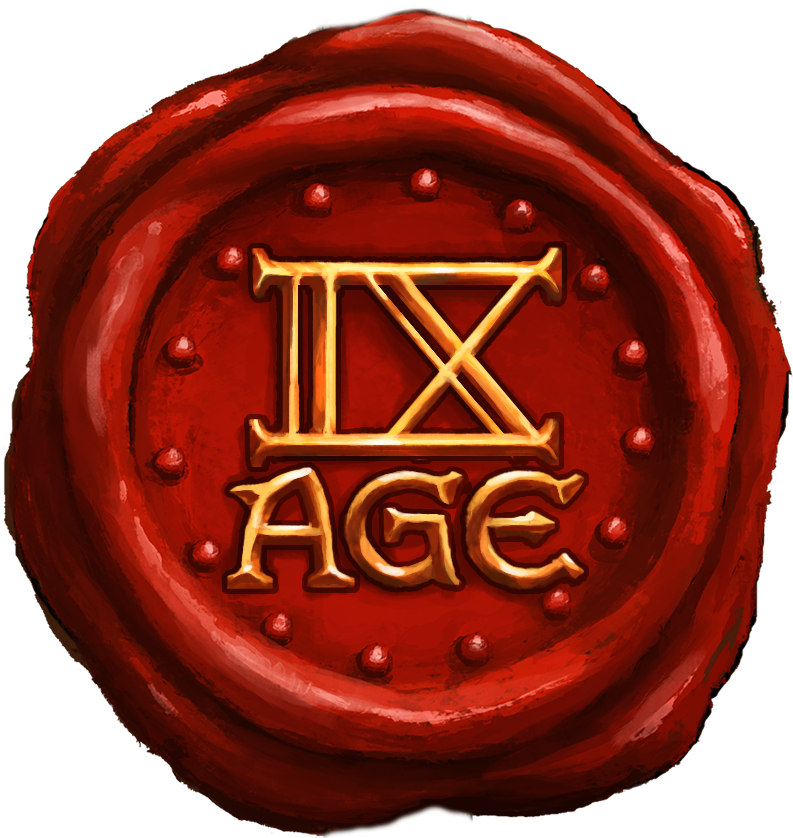
\includegraphics[width=2cm]{../Layout/pics/seal_9th.png} &
{\fontsize{10}{12}\selectfont \textcolor{black!50}{\noindent\labels@frontpagecredits}}

\ifdef{\frontpageaddstuff}{{\fontsize{10}{12}\selectfont \noindent\textcolor{black!50}{\frontpageaddstuff}}}{}

\vspace*{10pt}
\noindent{\fontsize{10}{12}\selectfont \textcolor{black!50}{\labels@license}}
\tabularnewline
\end{tabular}


\end{center}


\end{titlepage}

\restoregeometry

\clearpage
\section{Comment utiliser ce document ?}

Nous nous efforçons de vous fournir des documents de la meilleure qualité possible, mais des erreurs d'inadvertance ou des conséquences inattendues d'interactions entre les règles finissent toujours par apparaître. Cette Foire Aux Questions a été créée pour répondre à certaines questions parmi les plus posées ou les plus compliquées.

\section{Livre de Règles}

\questiontitle{Règle du Pouce d'Écart}{\pageref{unit_spacing}}

\QandA{%
À quelle distance des autres unités et des Terrains Infranchissables peuvent s'approcher les figurines qui se déplacent mais ne chargent pas ?
}{%
Les unités ne peuvent pas s'approcher à moins de 0,5\distance{} des autres unités ou des Terrains Infranchissables pendant un déplacement, et doivent finir leur mouvement à plus de \distance{1} de ceux-ci. Si une unité se trouve à moins de \distance{1} d'un obstacle avant de commencer à se déplacer (ce qui peut arriver après des mouvements de charge), elle ignore la Règle du Pouce d'Écart jusqu'à ce qu'elle soit à nouveau à plus de \distance{1}. Vous ne décalez jamais les unités dan ce cas.
}

\questiontitle{Utilisation des Caractéristiques non modifiées}{\pageref{unmodified_characteristics}}

\QandA{%
Quelles types de changement de Caractéristiques comptent pour les Caractéristiques non modifiées ?
}{%
Les améliorations faites lors de la construction de la Liste d'Armée qui ne sont pas des équipements (Objets Magiques, Armes, Armures, etc...) ne comptent pas comme des modificateurs et sont inclues dans les Caractéristiques non modifiées. Typiquement, les améliorations en \og vétérans \fg{} ou équivalent sont pris en compte pour obtenir les Caractéristiques non modifiées.
}

\questiontitle{Mouvement de charge}{\pageref{move_chargers}}

\QandA{%
Peut-on entrer en contact socle à socle avec plus d'une unité ennemie lors d'un Mouvement de charge ?
}{%
Oui, mais \textbf{uniquement} si il n'y a aucun autre moyen pour l'unité de réussir sa charge. L'unité en charge doit arriver au contact de la cible initiale avant d'entrer en contact avec une autre unité ennemie, ou entrer en contact avec les deux simultanément. Toute unité qui est chargée de cette manière doit déclarer une Réaction à la charge.
}

\questiontitle{Aligner les unités}{\pageref{aligning_units}}

\QandA{%
Un mouvement d'Alignement peut-il se faire à l'opposé de l'ennemi pour faire de la place pour l'unité ennemie en charge ?
}{%
Non. Un mouvement d'Alignement doit toujours se faire vers l'ennemi.
}

\questiontitle{Chemin bloqué}{\pageref{blocked_path}}

\QandA{%
Est-ce qu'un mouvement de Chemin bloqué peut mener une unité au contact de plusieurs ennemis ?
}{%
Oui. L'unité peut entrer au contact de plus d'une unité si un mouvement droit devant provoque cette situation. Ces unités seront alors chargées et feront toutes une Reformation de Combat pour les aligner à l'unité qui charge.
}

\questiontitle{Types de sorts}{\pageref{spell_types}}

\QandA{%
Un sort donnant la règle \frenzy{} la donne-t-il au cavalier et à sa monture ?
}{%
Oui. À moins que le contraire ne soit précisé, comme les sorts de type \focused{}, tous les effets des sorts sont appliqués à tous les éléments des figurines qu'ils ciblent.
}

\questiontitle{Distance et déplacement des unités en poursuite}{\pageref{pursuit_distance_and_pursuing_units}}

\QandA{%
Lorsqu'une unité en poursuite impacte une unité ennemie, à quel moment dois-je déterminer dans quel arc se trouve mon unité ?
}{%
Déterminez de quel coté de la cible la charge se fera avant le pivot initial. Ceci s'applique également pour les figurines avec la règle \randommovement{}.
}

\questiontitle{Personnage monté}{\pageref{character_mounts}}

\QandA{%
Un Personnage monté sur un \monster{} peut-il utiliser sa propre Sauvegarde d'Armure ?
}{%
Non. Les \riddenmonsters{} ne peuvent utiliser que la Sauvegarde d'Armure de la monture.
}

\questiontitle{Armes de Corps à Corps}{\pageref{close_combat_weapons}}

\QandA{%
Est-ce que les règles des Armes de Corps à Corps s'appliquent aux Armes spécifiques de Corps à Corps des Livres d'Armée ?
}{%
Oui. Cela signifie que les règles données pour toutes les Armes de Corps à Corps, du Livre de Règles et des Livres d'Armée, ne s'appliquent que lorsque l'arme en question est maniée. Elles ne s'appliquent pas aux Attaques Spéciales comme le \stomp{} ou quand une autre arme est utilisée. Notez que les bonus de Sauvegarde d'Armure offerts par des Armes de Corps à Corps fonctionnent aussi contre les Attaques à Distance.
}

\questiontitle{Catapulte (\distance{X})}{\pageref{catapult}}

\QandA{%
Quelle est la cible d'une Arme d'Artillerie de type \catapult{} ?
}{%
Toute unité qui se trouve au moins partiellement sous la position initiale du Gabarit est considéré comme étant ciblée par l'attaque. C'est principalement pertinent pour une unité qui possède plusieurs Attaques de Tir, dont une \catapult{} : toutes les figurines de l'unité doivent choisir la même cible, donc le Gabarit doit être au moins partiellement positionné au dessus de la cible.
}

\questiontitle{Distribuer les touches sur une Unité Combinée}{\pageref{distributing_hits_at_combined_units}}

\QandA{%
Un Champion compte-t-il comme une figurine ordinaire pour la répartition des touches sur un Personnage ?
}{%
Oui, ce qui signifie qu'un Champion et 4 figurines ordinaires classiques sont suffisantes pour protéger un Personnage.
}

\questiontitle{\frontrank{}}{\pageref{front_rank}}

\QandA{%
Certains Personnages peuvent perdre la règle \frontrank{}. Où puis-je le placer dans une unité ?
}{%
Les figurines qui perdent la règle \frontrank{} ignorent seulement le besoin d'être placées aussi à l'avant de l'unité que possible. Elles peuvent être placées n'importe où dans l'unité tant que les règles habituelles sur la formation des unités (un seul rang incomplet, pas de trous dans la formation, etc.) sont respectées. Les figurines avec la règle \frontrank{} ont la priorité pour le positionnement à l'avant de l'unité. Les autres règles concernant le fait d'avoir rejoint une unité, telles que bouger au sein d'une unité lors d'un Mouvement Simple, d'une Marche Forcée, d'une Reformation ou d'une Roue, ou encore comment retirer les pertes, la compatibilité des socles, etc., s'appliquent toujours.
}

\questiontitle{Faites Place}{\pageref{make_way}}
\QandA{%
Si une unité est chargée de flanc de telle sorte que l'avant de celle-ci est coin à coin avec l'ennemi, un Personnage peut-il utiliser la règle Faites Place ?
}{%
Non.
}

\questiontitle{Relever un Défi}{\pageref{fighting_a_challenge}}

\QandA{%
Si une figurine en Défi est retiré comme perte avant que son adversaire n'ai eu la possibilité d'attaquer, par exemple si cette figurine était un Champion dans une unité qui a été annihilée, l'adversaire peut-il quand même attaquer pour avoir le bonus de Carnage ?
}{%
Oui, tant que cette figurine a été retirée comme perte pendant la Phase de Corps à Corps.
}

\questiontitle{Champion}{\pageref{champion}}

\QandA{%
Peut-on Répartir des touches sur un Champion ?
}{%
Non, on ne peut pas répartir de touches sur un Champion. Notez bien la différence entre \og Répartir des touches \fg{} et \og Allouer des attaques \fg{}. Les touches sur les figurines ordinaires d'une unité avec un Champion sont réparties sur les figurines ordinaires non-Champion. Cela inclut les touches de Gabarit. Les Champions ne sont pas des Personnages, ils ne suivent donc pas les règles de répartition des touches sur les Personnages dans des unités. Les seules manières de tuer un Champion sont : un sort de type \focused{}, une attaque qui touche toutes les figurines d'une unité (comme le sort \naturespellsix{}) ou l'allocation d'attaques au Corps à Corps.
}

\questiontitle{Choisir le Général de l’armée}{\pageref{choosing_the_general}}

\QandA{%
Lorsque l'on choisit le Général de l’armée, on doit sélectionner la figurine avec le plus haut Commandement. Cela inclut-il les modificateurs ?
}{%
Oui, les modificateurs provenant des équipements ou des améliorations des figurines sont pris en compte pour choisir le Général. Toutefois, comme le Général est déterminé lors de la création de l'armée, les modificateurs qui sont appliqués uniquement dès le début de la bataille ne peuvent pas être utilisé. Cela inclut la modification du Commandement par des sorts et par le fait de rejoindre une unité qui transporte une Bannière de Discipline.
}

\questiontitle{Bâtiment}{\pageref{buildings}}

\QandA{%
Puis-je choisir de ne sélectionner aucune figurine pour les Assaillants ou les Défenseurs d'un combat dans un Bâtiment ?
}{%
Non. Vous devez choisir autant de figurines que possible selon le type de l'unité.
}

\questiontitle{\channel}{\pageref{channel_special_rule}}

\QandA{%
Est-ce que plusieurs instances de la règle \channel{} sur une même figurine s'additionne ?
}{%
Plusieurs instances de la règle sur un même élément de figurine n'ont pas d'effet additionnels par rapport à une seule instance. Cependant, deux éléments de figurine sur le même socle, tout deux avec la règle \channel{} (par exemple un Sorcier sur une monture qui est aussi un Sorcier), ajouteront deux +1 aux jets de \channel{} pour un total de +2.
}

\questiontitle{\daemonicinstability}{\pageref{daemonicinstability}}

\QandA{%
Comment l'\daemonicinstability{} interagit-elle avec les règles Indomptable et \stubborn{} ?
}{%
Une unité avec la règle \daemonicinstability{} qui possède aussi la règle \stubborn{} ou est Indomptable ne subira aucun modificateur négatif pour son test d'\daemonicinstability{} à cause du Résultat de Combat.
}

\questiontitle{\magicresistance{}}{\pageref{magicresistance}}

\QandA{%
Contre quels effets de sort fonctionne la \magicresistance{} ?
}{%
Seulement contre les dégâts générés directement par les sorts. Ça ne fonctionne pas contre les dégâts indirects des sorts, comme les règles données aux figurines qui causeront des dégâts plus tard. Par exemple, la \magicresistance{} ne donne aucun avantage contre les effets suivants :
\begin{itemize}[label={-}]
\item Les Attaques modifiées par les sorts (par exemple une figurine gagnant la règle \poisonedattacks{}).
\item Les Attaques Spéciales données à une figurine (par exemple, une figurine gagnant une \breathweapon{}).
\item Les tests de Terrain Dangereux entraînés par les sorts.
\end{itemize}
}

\questiontitle{\warplatform}{\pageref{warplatform}}

\QandA{%
Une \warplatform{} peut-elle rejoindre une unité avec un nombre impair de figurines au premier rang ?
}{%
Oui. Dans un tel cas il y a deux positions légales de placement au centre de l'unité, que vous pouvez choisir librement.
}

\questiontitle{Appliquer les règles spéciales}{\pageref{applying_special_rules}}

\QandA{%
Quelles règles spéciales modifiant les attaques s'appliquent aux Attaques de Tir, et lesquelles ne peuvent être utilisées qu'avec des Attaques de Corps à Corps ?
}{%
Il y a deux moyens d'appliquer les règles spéciales aux attaques. Si la règle est donnée spécifiquement à une arme, un sort ou une attaque (comme une \breathweapon{} ou des \impacthits{}), elle ne fonctionne qu'avec cette arme/sort/attaque. Si une figurine possède une règle spéciale, chaque règle spéciale possède ses propres règles d'applications. Par défaut elles ne s'appliquent qu'au Corps à Corps.

Cela signifie par exemple que la règle \poisonedattacks{} donnée par le sort \diseasespelltwo{} affectera les Attaques de Tir et de Corps à Corps, alors que la règle \lethalstrike{} donné par le sort \deathspellfive{} n'affectera que les Attaques de Corps à Corps. Notez que les effets qui ne sont pas des règles spéciales, tels que le \og +1 pour blesser \fg{} donné par le sort \firespelltwo{} affectent les Attaques de Tir et de Corps à Corps.
}

\questiontitle{Relever un Défi}{\pageref{fighting_a_challenge}}

\QandA{%
Des touches provenant d'une source extérieur au combat peuvent-elles être répartie sur une figurine étant en Défi ?
}{%
Oui. Seules les Attaques de Corps à Corps ne peuvent pas être réparties sur des figurines en Défi. Les Attaques provenant d'une source extérieur au combat (tir de Catapulte dévié, sorts qui permet de cibler une unité engagée au corps à corps, etc.) peuvent être réparties sur une figurine en Défi.
}

\questiontitle{Quitter une Unité Combinée}{\pageref{leaving_a_combined_unit}}

\QandA{%
Si un Personnage quitte une unité combinée en effectuant une Marche Forcée, et a passé le test de Marche Forcée, l'unité qu'il a quitté doit-elle aussi faire une Marche Forcée ? Doit-elle passer un nouveau test de Marche Forcée si elle souhaite en faire une aussi ?
}{%
Avant de passer un test de Marche Forcée, déclarez quelles figurines sont concernées par ce test. Cela peut être un Personnage, plusieurs Personnages, ou toute l'unité (Personnages et figurines ordinaires). Si le test a été passé pour des Personnages uniquement, et que tous ces Personnages quittent l'unité, les figurines restantes de l'unité sont libre d'effectuer d'autres actions, et doivent passer un nouveau test de Marche Forcée si elles souhaitent en faire une. Si certains Personnages ayant passé un test de Marche Forcée restent finalement dans l'unité, l'unité entière doit effectuer une Marche Forcée, et doit passer un test de Marche Forcée si elle ne l'a pas déjà fait.
}

\questiontitle{Distance et déplacement des unités en poursuite}{\pageref{pursuit_distance_and_pursuing_units}}

\QandA{%
Lorsqu'une unité en poursuite atteint une unité ennemie, elle doit déclarer une charge contre celle-ci. Que se passe-t-il lorsque cette charge est impossible à mener à bien ?
}{%
Aucune charge n'est déclarée.
}

\questiontitle{Capuche de Magicien}{\pageref{enchanted_items}}

\QandA{%
Que se passe-t-il si l'Objet Enchanté \og Capuche de Magicien \fg{} est détruit ?
}{%
Le porteur de l'objet perd la règle \stupidity{} et n'est plus un Sorcier, donc il ne peut plus lancer ni dissiper de sort, et n'a plus la règle \channel{}. Si il portait un Objet Magique que seul un Sorcier peut utiliser, comme un Parchemin de Dissipation (car seuls les Sorciers peuvent dissiper), il ne peut plus s'en servir.
}

\questiontitle{Bâtiment}{\pageref{buildings}}

\QandA{%
Comment cela se passe-t-il pour les figurines montées lors d'un Combat Multiple impliquant un Bâtiment ?
}{%
Seules les figurines choisies comme étant les Assaillants sont restreintes dans l'utilisation de \lance{}, \lightlance{} et \impacthits{}. La \mountsprotection{} et le \barding{} ne peuvent pas être utilisées contre les attaques provenant des Défenseurs du Bâtiment.
}

\questiontitle{Équipement Standard}{\pageref{mundane_equipment}}

\QandA{%
Qu'est-ce qui est compte comme arme et armure \og standard \fg{} ?
}{%
Toutes les armes et armures qui ne sont pas des Objets Magiques sont considérés comme standard.
}

\questiontitle{Priorité des Modificateurs}{\pageref{priority_of_modifiers}}

\QandA{%
Dans quel ordre les modificateurs de choses qui \textbf{ne} sont \textbf{pas} des Caractéristiques s'appliquent-ils ?
}{%
Ils s'appliquent en utilisant le même ordre de priorité que les modificateurs de Caractéristiques (p. \pageref{priority_of_modifiers}).

Par exemple, les Globes de Gaz Nocif de la Marée de Vermine blesse toujours sur 4+. Si cette attaque subit un modificateur de -1 pour blesser, elle blesse sur 5+ puisque la soustraction prend effet après que la valeur est fixée à une certaine valeur.
}

\questiontitle{Fiasco}{\pageref{miscast}}

\QandA{%
Lorsqu'un résultat de \result{8} ou \result{9} (\sorcerousbacklash{}) est obtenu, combien de touches subit une figurine composée de plusieurs Sorciers (par exemple un Sorcier monté sur une monture qui est également un Sorcier) ?
}{%
Une touche par élément de figurine qui est un Sorcier.
}

\questiontitle{\catapult{}}{\pageref{catapult}}

\QandA{%
Lorsque l'on tire avec une Arme d'Artillerie de type \catapult{} et que l'on obtient un \og Touché ! \fg{}, peut-on ne pas lancer le dé donnant la distance dont le Gabarit aurait dévié ?
}{%
Non. Le dé pour la distance de déviation du Gabarit doit toujours être lancé, car il sert à déterminer si la Catapulte subit un Incident de Tir.
}



\clearpage
\section{Livre de Magie}

\setcounter{Qcounter}{0}

\questiontitle{\Pathof{} \whitemagic{} : \whitemagicattribute}{\pageref{white_magic}}

\QandA{%
Que deviennent les marqueurs Bouclier quand un Personnage rejoint ou quitte une unité ?
}{%
Voici les différentes possibilités :
\begin{itemize}[label={-}]
\item Un Personnage \textbf{avec} un marqueur Bouclier rejoint une unité \textbf{avec} un marqueur Bouclier : Retirez un marqueur Bouclier. Le Personnage et l'unité peuvent utiliser le marqueur Bouclier restant.
\item Un Personnage \textbf{sans} marqueur Bouclier rejoint une unité \textbf{avec} un marqueur Bouclier : Le Personnage et l'unité peuvent utiliser le marqueur Bouclier.
\item Un Personnage \textbf{avec} un marqueur Bouclier rejoint une unité \textbf{sans} marqueur Bouclier : Le Personnage et l'unité peuvent utiliser le marqueur Bouclier.
\item Un Personnage quitte une unité \textbf{avec} un marqueur Bouclier : \textbf{Choisissez qui garde le marqueur} entre l'unité et le Personnage. L'autre n'a plus de marqueur.
\end{itemize}
}



\clearpage
\section{Livres d'Armée}

\subsection{Anciens Sauriens}
\setcounter{Qcounter}{0}

%\questiontitle{Sarbacane}{\pageref{blowpipe}}
%
%\QandA{%
%Est-ce qu'une Sarbacane gagne +1 pour toucher sur une unité qui contient un Personnage avec la règle \largetarget{} (certaines \warplatforms{} ont \largetargets{}) ?
%}{%
%Non. Toutes les figurines de l'unité doivent avoir la règle \largetarget{} pour que la Sarbacane bénéficie de +1 pour toucher.
%}


\subsection{Conclaves Vampiriques}
\setcounter{Qcounter}{0}

%Anneau d’Éternité (p6)
%Q1 : Qu'est-ce que ça signifie d'être immunisé aux règles \lethalstrike{} et \multiplewounds{}{} ?
%R1 : Ça signifie que les attaques dirigées contre le porteur de l'Anneau d’Éternité perdent les règles \lethalstrike{} et \multiplewounds{}{}.


\subsection{Dynasties Immortelles}
\setcounter{Qcounter}{0}

%Grand Arc Aspic (p2)
%Q1 : Une figurine avec un Grand Arc Aspic peut-elle choisir d'utiliser une \hw{} normale au corps à corps ?
%R1 : Non.


\subsection{Elfes Sinistres}
\setcounter{Qcounter}{0}

\questiontitle{Dague de Moraec}{\pageref{dread_elves_magical_items}}

\QandA{%
À quel moment la Dague de Moraec peut être utilisée ?
}{%
Elle doit être utilisée avant de lancer un sort. La Dague de Moraec ne peut pas être utilisée pour réduire la valeur de lancement d'un sort après avoir lancé les Dés de Pouvoir pour ce sort.
}


\subsection{Guerriers des Dieux Sombres}
\setcounter{Qcounter}{0}

%Marques des Dieux Sombres (p1)
%Q1 : Comment les Marques des Dieux Sombres intéragissent avec les Personnages rejoignant les unités ?
%R1 : Un Personnage peut rejoindre n'importe quelle unité, tant que celle-ci ne contient pas de figurine avec une Marque différente de celle du Personnage. La Marque du Chaos Intégral est une exception à cette règle, et n'empêche jamais un Personnage de rejoindre cette unité, quelque soit la Marque du Personnage. De même, un Personnage avec la Marque du Chaos Intégral peut rejoindre n'importe quelle unité, quelque soit sa Marque.


\subsection{Harde Bestiale}
\setcounter{Qcounter}{0}

\questiontitle{Icône du Pillard}{\pageref{beast_herds_magical_items}}

\QandA{%
Une unité composé de plus d'un Dent-Tranchante peut-elle utiliser la règle \vanguard{} lorsqu'elle se situe à moins de \distance{12} de l'Icône du Pillard ?
}{%
Oui. Seuls les \chariots{} sont limités à une figurine par unité pour profiter de l'Icône du Pillard.
}

\questiontitle{Peau Écorchée d’Aaghor}{\pageref{beast_herds_magical_items}}
\QandA{%
Une figurine sur un \chariot{} peut-elle prendre la Peau Écorchée d’Aaghor ?
}{%
Non. Le \chariot{} a une \mountsprotection{} qui est considérée comme une Armure.
}


\subsection{Khans Ogres}
\setcounter{Qcounter}{0}

%Coeur Démoniaque (p3)
%Q1 : Est-ce que le Coeur Démoniaque cause aux Sorciers ennemis un Fiasco lorsqu'un double arrive quelque soit le résultat final ?
%R1 : Oui. Cet objet cause un Fiasco si n'importe quel double est tiré, que le sort soit un succès ou un échec, dissipé (en utilisant des Dés de Dissipation ou un Parchemin de Dissipation) ou non.


\subsection{Royaume d'Équitaine}
\setcounter{Qcounter}{0}

%Serment d’Allégeance (p2)
%Q1 : Des unités avec des figurines ayant la règle \insignificant{} et des figurines sans la règle \insignificant{} relancent-elles les tests de Commandement lorsqu'elles sont à \distance{6} d'une figurine avec Humilité ?
%R1 : Non. Toutes les figurines de l'unité doit avoir la règle \insignificant{} pour pouvoir relancer leurs tests de Commandement.
%
%Voeux de la Quête (p2)
%Q2 : Les Personnages avec les Voeux de la Quête ne peuvent pas "utiliser" d'autres armes que des \gw{}. Qu'est-ce que ça veut dire ?
%R2 : Que t'es trop con pour jouer au 9e age, va jouer a AoS et meurt.
%Les Personnages avec les Voeux de la Quête ne peuvent se servir des armes qu'ils portent qui ne sont pas des \gw{}, en aucun cas.
%
%Archers Paysans {p9}
%Q3 : Les Archers Paysans peuvent-ils prendre une \crossbows{} dans une armée contenant des Frères Pénitents ? (ndlr : cette question se pose à cause des noms VO, qui ne pose aucun problème en VF)
%R3 : Non. L'amélioration requière "Croisés", se référant à l'amélioration de l'unité Aspirants Paladins.


\end{document}
